\documentclass[11pt]{article}

%	packages
\usepackage{amsmath}
\usepackage{amssymb} 
\usepackage{caption}
\usepackage{graphicx}
\usepackage{authblk}
\usepackage[hypertexnames=false,colorlinks=true,linkcolor=blue,citecolor=blue]{hyperref}
\usepackage[numbers,comma,square,sort&compress]{natbib}
\usepackage[a4paper,text={6.5in,10in},centering]{geometry}
\usepackage{subcaption}
\usepackage{tikz}
\usetikzlibrary{arrows}
\usetikzlibrary{decorations.markings}
\usepackage{pgfplots}
\usetikzlibrary{calc}
\usetikzlibrary{matrix}
\tikzstyle{code} = [rectangle, minimum width=1cm, minimum height=0.5cm, text centered, rounded corners, draw=black, fill=gray!30]
\tikzstyle{user} = [rectangle, minimum width=1cm, minimum height=0.5cm, text centered, rounded corners, draw=black, fill=lbcolor]
\tikzstyle{iterative} = [red!80]
\newcommand{\midarrow}{\tikz \draw[-stealth'] (0,0) -- +(.1,0);}
\newcommand{\midarrowThick}{\tikz \draw[-stealth', thick] (0,0) -- +(.1,0);}
%	code syntax higlighting
\usepackage{listings}
\usepackage{color}
\usepackage{textcomp}
\usepackage{algpseudocode}
\usepackage{algorithm}
\definecolor{listinggray}{gray}{0.9}
\definecolor{lbcolor}{rgb}{0.9,0.9,0.9}
% C++ = [Visual]C++ ; matlab = matlab
\lstset{
	backgroundcolor=\color{lbcolor},
	tabsize=4,
	rulecolor=,
	language=java,
	keywordstyle=\bfseries\ttfamily\color[rgb]{0,0,1},
	identifierstyle=\ttfamily,
	commentstyle=\color[rgb]{0.133,0.545,0.133},
	stringstyle=\ttfamily\color[rgb]{0.627,0.126,0.941},
	showstringspaces=false,
	basicstyle=\small,
	%numberstyle=\footnotesize,
	%numbers=left,
	stepnumber=1,
	numbersep=10pt,
	tabsize=2,
	breaklines=true,
	prebreak = \raisebox{0ex}[0ex][0ex]{\ensuremath{\hookleftarrow}},
	breakatwhitespace=false,
	aboveskip={1.5\baselineskip},
  columns=fixed,
  upquote=true,
  extendedchars=true,
 frame=single,
% backgroundcolor=\color{lbcolor},
}


%	layout
\setlength{\parindent}{0.0in}
\setlength{\parskip}{1.0ex plus0.2ex minus0.2ex}
\renewcommand{\baselinestretch}{1.2}

%	figures
\graphicspath{{eps/}{pdf/}{Figures/}{../BMC2015/figures/}}
%\setcaptionmargin{0.25in}
\def\captionfont{\itshape\small}
\def\captionlabelfont{\upshape\small}

%	counters
\makeatletter\@addtoreset{equation}{section}\makeatother
\renewcommand{\theequation}{\arabic{section}.\arabic{equation}}

%	environments
\newtheorem{Lemma}{Lemma}[section]
\newtheorem{Theorem}{Theorem}
\newtheorem{Proposition}[Lemma]{Proposition}
\newtheorem{Corollary}[Lemma]{Corollary}
\newtheorem{Remark}[Lemma]{Remark}
\newtheorem{Definition}[Lemma]{Definition}
\newtheorem{Hypothesis}[Lemma]{Hypothesis}

\newenvironment{Proof}%
 {\begin{trivlist} \item[]{\bf Proof. }}%
 {\hspace*{\fill}$\rule{.4\baselineskip}{.4\baselineskip}$\end{trivlist}}

\newenvironment{Acknowledgment}%
 {\begin{trivlist}\item[]\textbf{Acknowledgments.}}{\end{trivlist}}

\def\Fix{\mathop\mathrm{Fix}\nolimits}

\newcommand{\R}{\mathbb{R}}
\newcommand{\C}{\mathbb{C}}
\newcommand{\N}{\mathbb{N}}
\newcommand{\Z}{\mathbb{Z}}

\def\Re{\mathop{\mathrm{Re}}}
\def\Im{\mathop{\mathrm{Im}}}

\newcommand{\rmO}{\mathrm{O}}
\newcommand{\rmo}{\mathrm{o}}
\newcommand{\rmd}{\mathrm{d}}
\newcommand{\rme}{\mathrm{e}}
\newcommand{\rmi}{\mathrm{i}}
\newcommand{\im}{\mathrm{Im}\,}
\renewcommand{\ker}{\mathrm{Ker}\,}
\newcommand{\id}{\mathrm{\,id}\,}
\newcommand{\ad}{\mathrm{ad}}
\newcommand{\Rg}{\mathrm{Rg}}

% Gaussian
\pgfmathdeclarefunction{gauss}{3}{%
  \pgfmathparse{#3*1/(#2*sqrt(2*pi))*exp(-((x-#1)^2)/(2*#2^2))}%
}

\newcommand*\mean[1]{\overline{#1}}


\begin{document}

\title{Equation-free analysis of agent-based models: systematic parameter determination}

\author[1]{Spencer A. Thomas}
\author[1]{David J.B. Lloyd}
\author[1]{Anne C. Skeldon}
\affil[1]{\small Department of Mathematics, University of Surrey, Guildford, GU2 7XH, UK}
\date{\today}
\maketitle

\renewcommand{\vec}[1]{\mathbf{#1}}



\section{Time horizon $\tau$}
\label{sec:parametersTau}

For deterministic systems, an ensemble of microscopic models initialised at the same state, will  
all be in the same state after a simulation time of $\tau$. Stochastic systems however, will 
result in distribution of final states with a mean $\bar{x}$ and variance $\sigma^2\neq0$. 
The value of $\sigma^2$ will vary due to the dynamics and the noise of the system, as may $\bar{x}$, and thus depends on the size of the time evolution. For increasing time windows, $\sigma^2$ may either;
\begin{enumerate}
\label{list:tauType}
\item increase indefinitely with $\tau$ (diffusion in an open system), 
\item increase to a point then remain approximately constant (point of balance or symmetry in the system), or
\item increase to a maximum point then begin to reduce (transition from one state to another). 
\end{enumerate}

\begin{figure}[h]
	\centering
	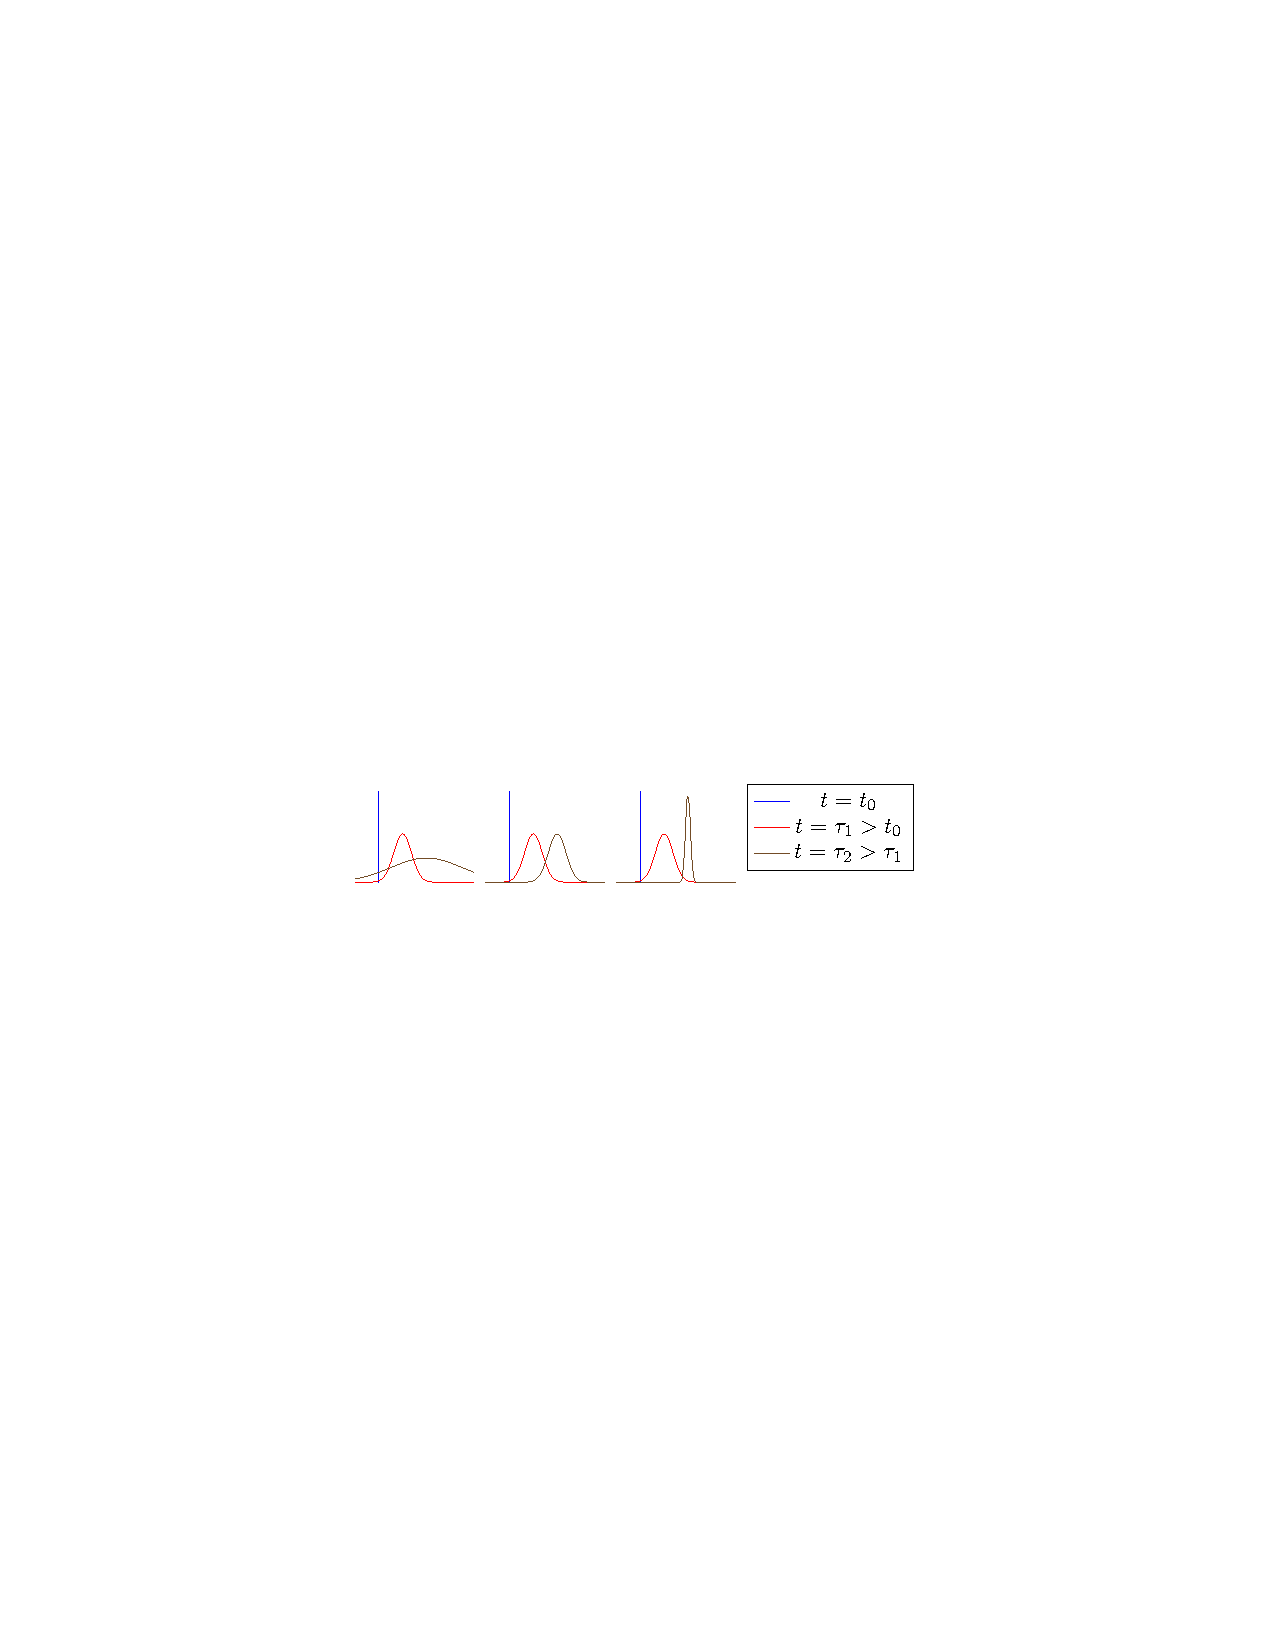
\includegraphics[width=0.8\textwidth, trim= 6cm 13cm 6cm 13cm, clip=true]{GaussianPlots}
	\caption{Dependence of $\sigma^2$ on $\tau$. For increasing $\tau$, $\sigma^2$ increases; indefinitely (left), to a constant (mid), or to a maximum before reducing (right). \label{fig:tauPredictor}}
\end{figure}


This is illustrated in Fig.~\ref{fig:tauPredictor}. For an arbitrary system, the distribution of 
an ensemble of simulation, the realisations, at $\tau$ is unknown, and although we can simply calculate $\bar{x}$, we can not calculate $\sigma^2$ in general. We can however average a number of ensembles resulting in a distribution 
of $\bar{x}$ which, according to the central limit theorem (CLT) is normally distributed. From the 
distribution of $\bar{x}$ we can calculate a mean $\overline{\bar{x}}$ (the mean of the means) and a 
standard deviation $\omega$. As increasing $\tau$ leads to an increase, at least initially, in
$\bar{x}$ and $\sigma^2$, it will also effect $\overline{\bar{x}}$ and $\omega$. By defining a a minimum 
threshold $\gamma$ for the value of $\omega$, which reflects the amount of variation across the ensembles, 
we can obtain a value of $\tau$ that enables sufficient time evolution such that the dynamic behaviour in
the model is observable. That is, increase $\tau$ until $\omega \geq \gamma$. This provides a platform for 
the systematic determination of $\tau$ for a specific model, avoiding excessive trial and error testing, or the need of a deterministic equivalent. This process is illustrated in Fig.~\ref{fig:tauGamma} 
and the procedure is summarised in Algorithm~\ref{algorithm:tau}. 







\begin{algorithm}[h]
	\caption{Time horizon predictor. \label{algorithm:tau}}
	\begin{algorithmic}
		\State \textcolor{blue}{\# obtain initial parameter settings}
		\State $N=N_{int}$ \textcolor{blue}{\# initial realisations (default=10)}
		\State $\tau=\tau_{int}$ \textcolor{blue}{\# initial time horizon}
		\State $\delta\tau$ \textcolor{blue}{\# time horizon increment}
		\State $M$ \textcolor{blue}{\# number of runs to average over}
		\State $MaxIter$ \textcolor{blue}{\# maximum number of iterations}
		\State $\gamma$ \textcolor{blue}{\# threshold for dynamics}
		\While {$iterations < MaxIter$}
			\For {$j=0;j<M$}
				\State $LIFT(N)$
				\State $SIMUALTE(N,\tau)$
				\State $\bar{\vec{x}}[j] = RESTRICT(N)$
				\State j := j+1
			\EndFor
		%	\State \textcolor{blue}{\# mean, variance and 95 \% confidence interval of means}
		%	\State {$\overline{\bar{x}}$} = AVE({$\bar{\bf x}$}) 
		%	\State {$\omega_i$} = VAR({$\bar{\bf x}$}) 
		%	\State {${\phi}$} = STDERR({$\bar{\bf x}$}) * 1.96 
			\State \textcolor{blue}{\# 95 \% confidence interval of distribution of means}
			\State {$\omega_i$} = 95ConfInt({$\bar{\bf x}$})
		
		%	\If {$0.9{\omega}_{j-1} > {\omega}_j$} 
		%		\State PRINT: seeing `less dynamics', reduce $\delta \tau$ 
		%	\EndIf
		%	\If {$0.9{\omega}_{j-1} < {\omega}_j  < 1.05{\omega_j}$} 
		%		\State PRINT: additional dynamics may not be worth the extra computational time
		%	\EndIf
			\If {$\omega > \gamma$} 
				\State EXIT \textcolor{blue}{\# $\tau$ large enough to see some dynamics}
			\EndIf
			\State $\tau$ := $\tau * \delta\tau$
			\State iterations := iterations + 1
		\EndWhile

\end{algorithmic}
\end{algorithm}

\begin{figure}[h]
	\centering
	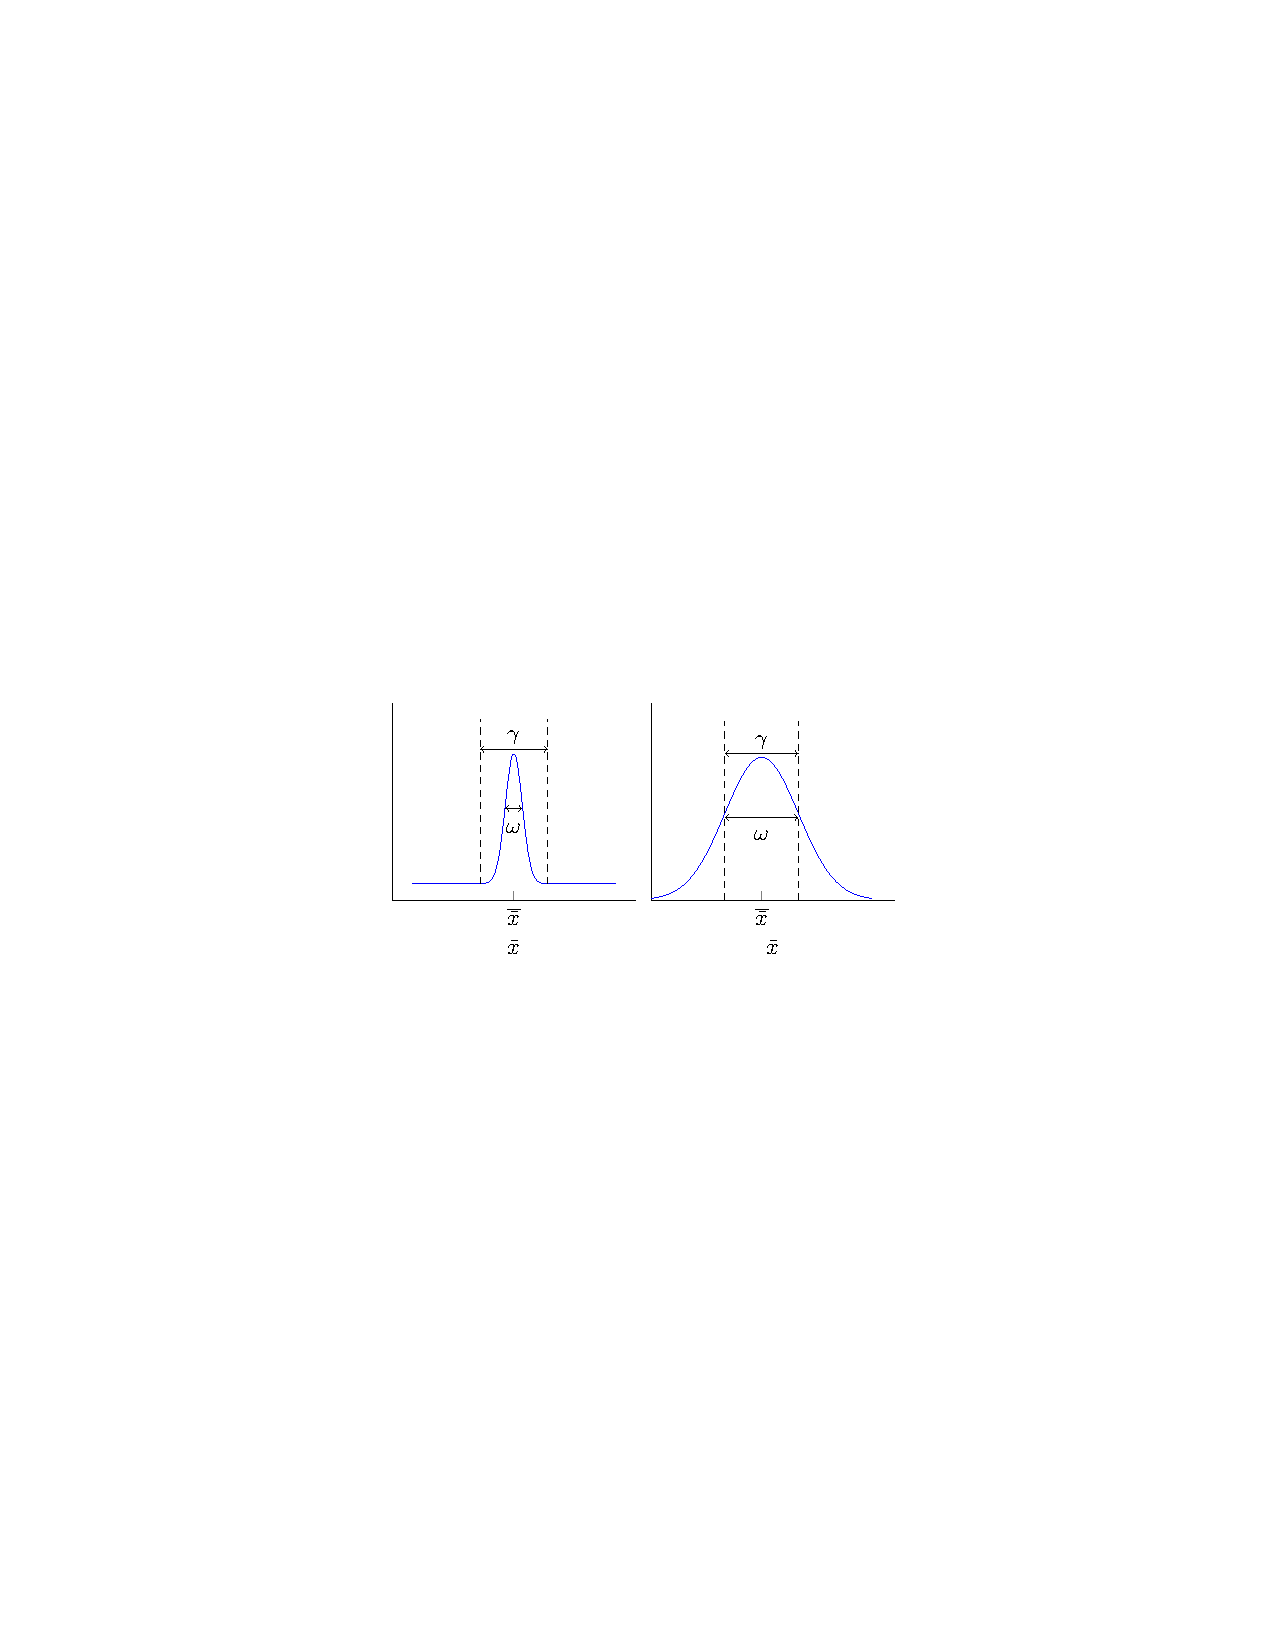
\includegraphics[width=0.8\textwidth, trim= 6cm 11.5cm 6cm 12cm, clip=true]{PredictionTau}
	\caption{Variance of the distribution of means, $\omega$ with $\gamma$ limit. For small $\tau$ (left) $\omega<\gamma$, whereas for larger $\tau$ (right) $\omega\approx\gamma$. \label{fig:tauGamma}}
\end{figure}


\section{Number of microscopic realisations $N$}
\label{sec:parametersN}

% In breif
Once we have obtained a value for the time evolution of the microscopic simulations we can then obtain a prediction for the number of microscopic realisations required to perform EF continuation of a generic ABM. The time horizon predictor in Algorithm~\ref{algorithm:tau} provides both a prediction of $\tau$ and a measure of how well defined this value is through $\omega_N$, which we can use as our threshold in the realisation predictor. That is, we can again use the CLT to obtain a (Gaussian) distribution of means and calculate the mean of means, variance and confidence interval. Here we can use the value of $\omega$ from the time horizon predictor as a limit for the variance of the distribution of means for the realisations, i.e. $\omega_{N}$. This process is summaries in Algorithm~\ref{algorithm:N}.  

\begin{algorithm}[h!]
	\caption{Realisation predictor. \label{algorithm:N}}
	\begin{algorithmic}
		\State \textcolor{blue}{\# obtain initial parameter settings}
		\State $N=N_{int}$ \textcolor{blue}{\# initial realisations}
		\State $\delta N$ \textcolor{blue}{\# increment in $N$}
		\State $M$ \textcolor{blue}{\# number of runs to average over}
		\State $N_{Max}$ \textcolor{blue}{\# maximum number of realisations}
		\State $\tau$ \textcolor{blue}{\# time horizon from Algorithm~\ref{algorithm:tau}}
		\State $\gamma$ \textcolor{blue}{\# threshold for dynamics from Algorithm~\ref{algorithm:tau}}
		\While {$\omega_N > \gamma$}
			\For {$j=0;j<M$}
				\State $LIFT(N)$
				\State $SIMUALTE(N,\tau)$
				\State $\bar{\vec{x}}[j] = RESTRICT(N)$
				\State j := j+1
			\EndFor
		%	\State \textcolor{blue}{\# mean, variance and 95 \% confidence interval of means}
		%	\State {$\overline{\bar{x}}$} = AVE({$\bar{\bf x}$}) 
		%	\State {$\omega_i$} = VAR({$\bar{\bf x}$}) 
		%	\State {${\phi}$} = STDERR({$\bar{x}$}) * 1.96 
			\State \textcolor{blue}{\# 95 \% confidence interval of distribution of means}
			\State {$\omega_N$} = 95ConfInt({$\bar{\bf x}$})
			%			
			\State $N := N * \delta N$
			%\State $N$ = RoundSigFig($N,k$) \textcolor{blue}{\# round (up) $N$ to $k$ significant figures (optional)}
			%\If {$N>=N_{MAX}$}
			%	\State PRINT: Large $N$ my cause large run times, suggest changing $\gamma$ or $\delta N$
			%	\State EXIT
			%\EndIf
		\EndWhile
\end{algorithmic}
\end{algorithm}



\section{Continuation step size $\delta s$ and finite differencing}
\label{sec:parametersDs}

We require a step size ($\delta s$), in the continuation parameter $\lambda$ such that if $f(x^\ast,\lambda) = x^\ast$, then $f(x^\ast,\lambda+\delta s) \approx x^\ast$. That is, we require $\delta s$ to be small enough so that we obtain a suitable prediction to $f$ under this perturbation. However this cannot be arbitrary small due to finite computational resources, impractical run times, and will depend on the specific problem under investigation. As with $N$ and $\tau$, for $\delta s$ we can determine a value based directly on simulation of the system. In this case by examining the level for stochasticity through the variance using the parameter obtained with Algorithms~\ref{algorithm:tau} and \ref{algorithm:N}. We perform the {\it Lift} and {\it Simulation} operations for one set of realisations and calculate the standard error in the mean ($\Delta$) of the distribution of simulation results. We then simply define the the step size as 
\begin{equation}
	\delta s = 3 \Delta~.
	\label{eq:ds}
\end{equation}

%a suitable prediction for the fixed point under the perturbation $\lambda \rightarrow \lambda + \delta s$ from $f(\tilde{x},\lambda)$, such that the prediction is suitably close to the actual solution. This cannot be arbitrary small due to finite computational resources and will depend on the specific problem under investigation, and also will lead to impractical run times. As with $N$ and $\tau$, for $\delta s$ we can make an initial prediction based directly on simulation of the system, in this case by examining the level for stochasticity through the variance. For the parameter obtained using Algorithms~\ref{algorithm:tau} and \ref{algorithm:N} we perform the {\it Lift} and {\it Simulation} operations for one set of realisations and calculate the standard error in the mean of the distribution of simulation results. We can use the standard error ($\Delta$) and finite differencing to define the step size used in the calculation of the Jacobian, $J$, 

During the predictor-corrector continuation used here, it is common to employ a Newton-Rhapson corrector method. In order to determine the update step size in this procedure we use finite differencing to calculate the Jacobian $J$,
\begin{equation}
	J_{ik} = \frac{f_i(x+h) - f_k(x)}{h}~,
	\label{eq:Jacobian}
\end{equation}
for $i,k = 0 \dots m$, where $m$ is the number of orders in $f$. The result of Eq.~(\ref{eq:Jacobian}) is an $m \times m$ matrix. The value $h$ is also problem specific as the accuracy of the determination of $J$ will depend on the magnitude of $h$ compared to $x$. To ensure that $J$ is accurately calculated for a general system, we define the value of $h$ in terms of the continuation step size,
\begin{equation}
	h = \frac{\delta s}{r}~,
	\label{eq:h}
\end{equation}
where $r=2$ in this work. 
%Here we define $h=3\Delta$. This value of $h$ ensures that $f(x+h)$ and $f(x)$ are unlikely to be from the same distribution, thus enabling the computation of the Jacobian and convergence of the fixed point. With regards to the continuation step size, we wish to make a predictions such that we are sufficient far from the previous converged value, but that the prediction is still close to the actual solution. Therefore we simply define the $\delta s = 2h$, and thus can obtain a prediction for the continuation step size directly from simulations of the system. A illustration of this is given in Fig~\ref{fig:dsPredictor}. This procedure enables the determination of a minimum value for $\delta s$ and giving the user an indication as to the order of magnitude for the step size, which they can experiment with if desired.

\begin{figure}[t]
	\centering
	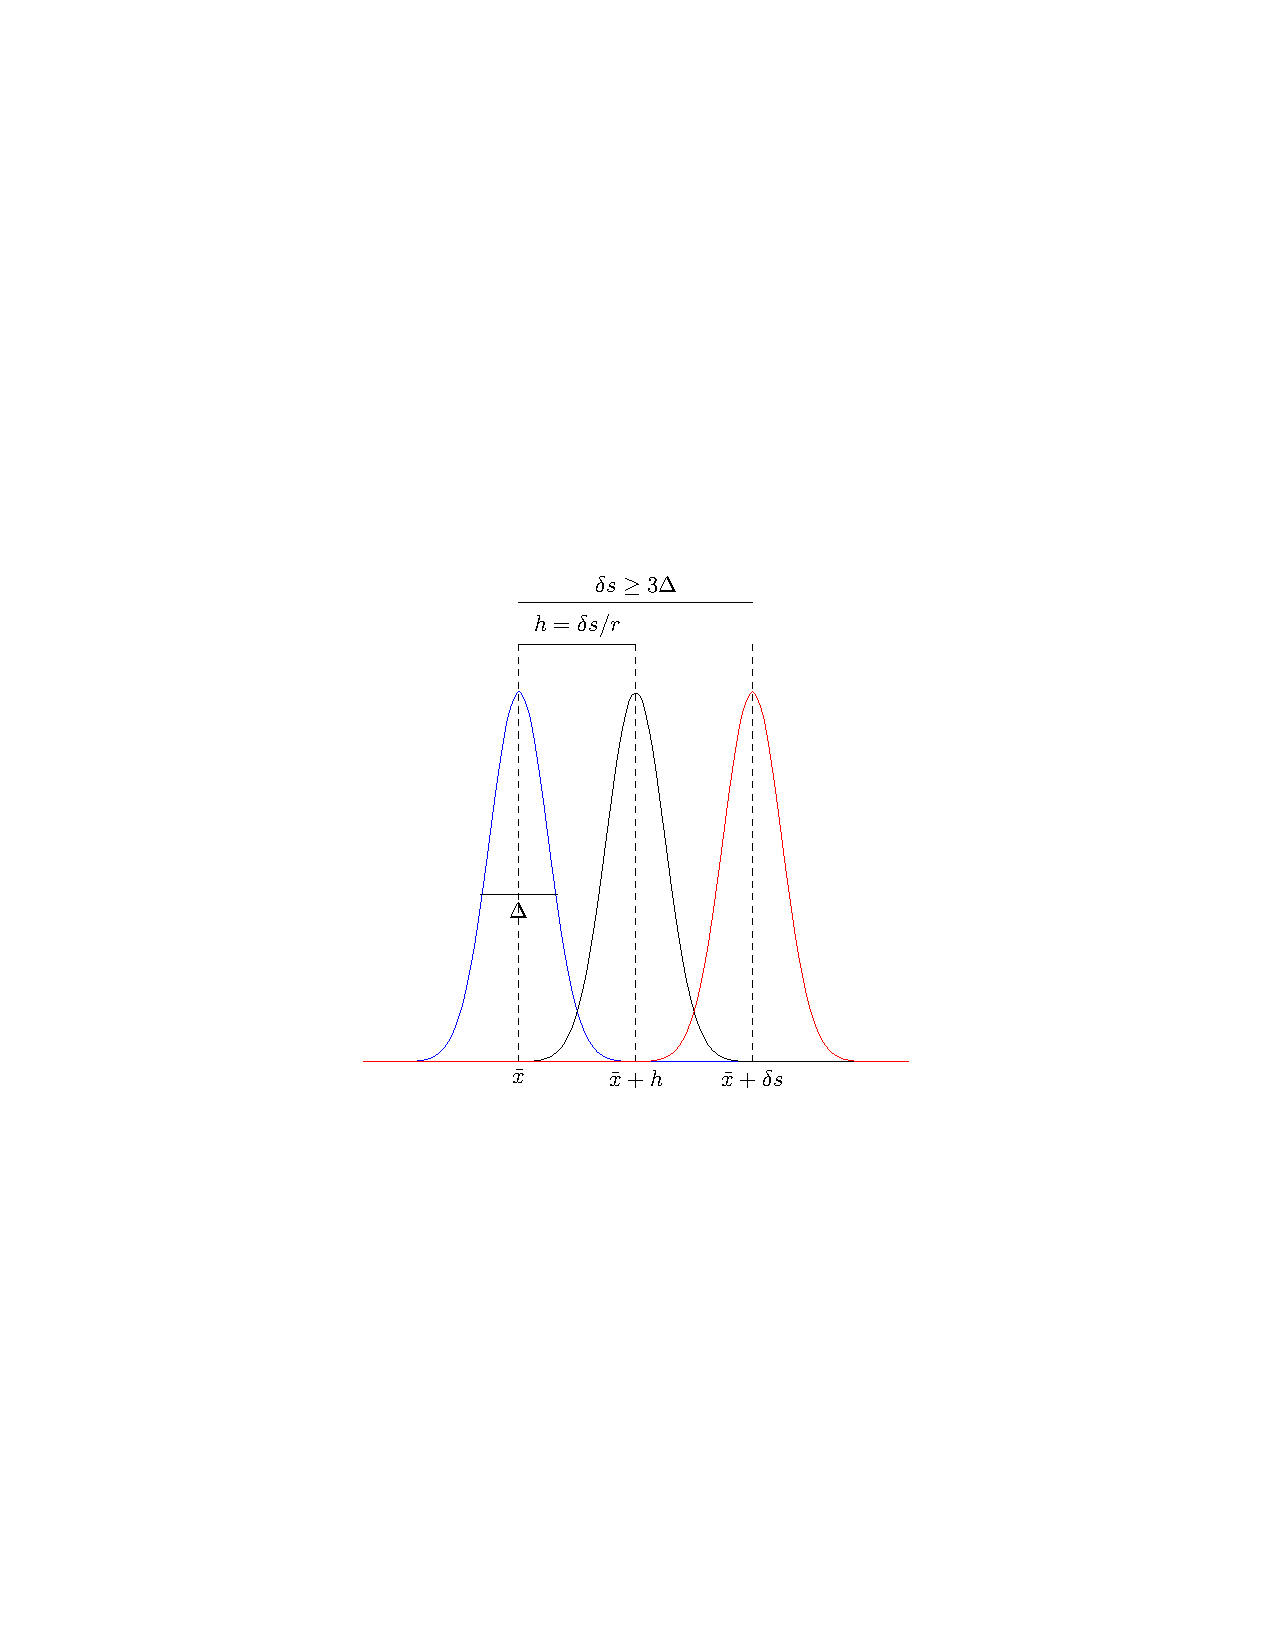
\includegraphics[width=0.5\textwidth, trim = 6cm 9cm 6cm 9cm, clip=true]{PredictionDS}
	\caption{Illustration of the $\delta s$ predictor. The standard error ($\Delta$) from the the simulation of $N$ realisations (blue) is used to determine the step size for finite differencing (black) and continuation step size (red). \label{fig:dsPredictor}}
\end{figure}



\section{Iterative determination and the selection of $\gamma$} 

It is worth noting that the value of $\gamma$ in Algorithm~\ref{algorithm:tau} and \ref{algorithm:N} is technically a tunable, problem specific parameter. However, here we have replaced three problem specific parameters with a single parameter, thus reducing the overhead. We note however that $\gamma$ can easily be obtained for a arbitrary model. By perform the procedure in Algorithm~\ref{algorithm:tau} with an arbitrarily large $\gamma$ (say 10,000) one can monitoring $\omega$ as a function of $\tau$. The profile of this curve can be used to select a new value of $\gamma$ for the specific model and Algorithm~\ref{algorithm:tau} can be repeated. Figure~\ref{fig:omega} shows the dependence of $\omega$ on $\tau$ when using an arbitrarily large $\gamma$. Here we can see that we can use these curves to obtain a better guess for $\gamma$ and obtain our problem specific equation-free parameters. 

	\begin{figure}
		\centering
		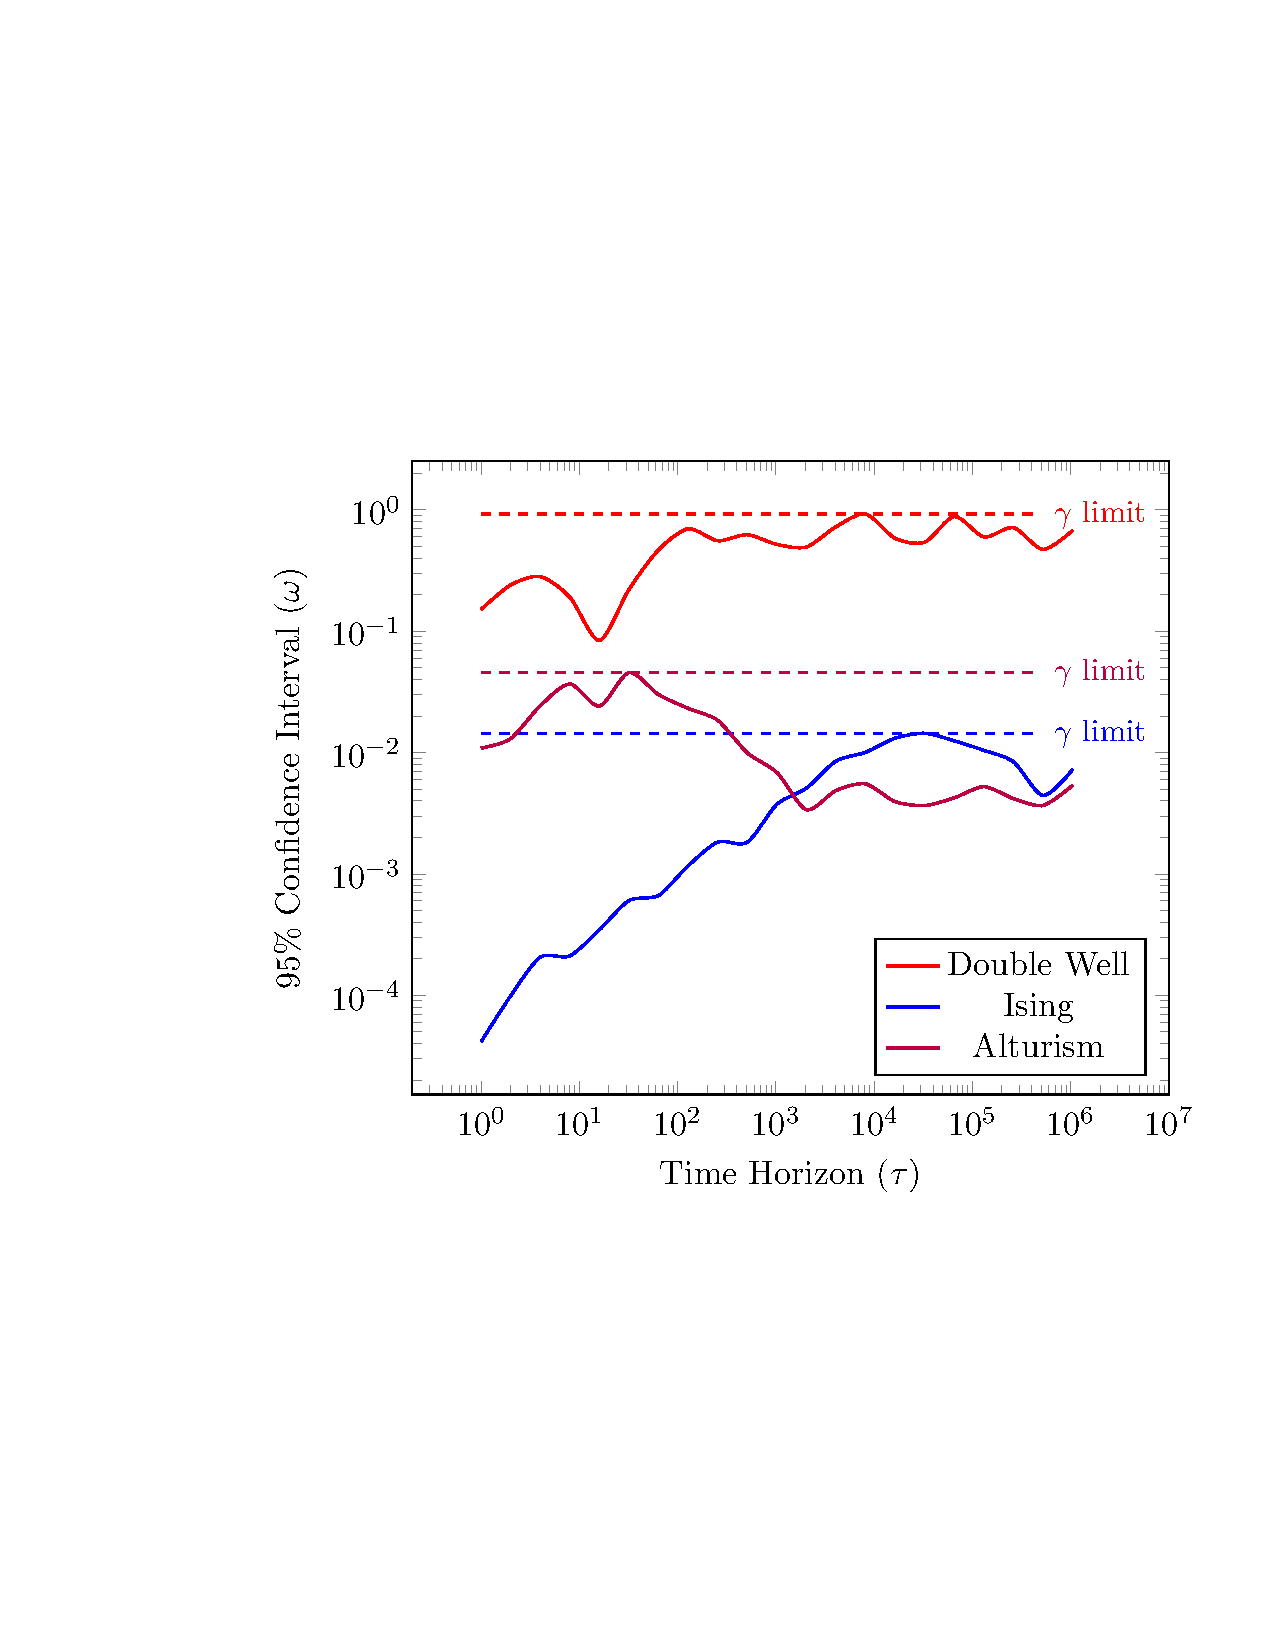
\includegraphics[width=0.82\textwidth, trim= 4cm 7cm 0cm 7cm, clip=true]{omega}
		\caption{Confidence interval on mean of $g(x)$ for 3 examples from the Repository of Models showing the maximum value of $\gamma$ in each case. \label{fig:omega}}
	\end{figure}	


\section*{Acknowledgements}
{The support of the UK Engineering and Physical Sciences Research Council for programme grant EP/H021779/1 (Evolution and Resilience of Industrial Ecosystems (ERIE)) is gratefully acknowledged.}
 
 


\end{document} 
